\documentclass{llncs}
%
\usepackage{makeidx}  % allows for indexgeneration
\usepackage{float}
%
\usepackage{textcomp}
\usepackage[T1,T2A]{fontenc}                    % Поддержка русских букв
\usepackage[utf8]{inputenc}[2014/04/30]         % Кодировка utf8
\usepackage[english, russian]{babel}[2014/03/24]% Языки: русский, английский
\usepackage{indentfirst}
\usepackage{graphicx} % Allows including images
\usepackage{booktabs} % Allows the use of \toprule, \midrule and \bottomrule in tables
\usepackage{caption}
\usepackage{amsmath}
\usepackage{amsFonts}
\usepackage{textcomp}
\usepackage{xcolor}
\usepackage{multirow}
\usepackage{geometry}   % Для последующего задания полей
\usepackage{times,a4wide}

\sloppy

\bibliographystyle{splncs03}
%
\begin{document}
\mainmatter              % start of the contributions
%
\title{\hbox{\normalsize УДК 519.8}Алгоритм дифференциальной эволюции для оптимизации направленности фазированных антенных решеток}
%
\titlerunning{ }  % abbreviated title (for running head)
%                                     also used for the TOC unless
%                                     \toctitle is used
%
\author{Еремеев А.В.\inst{1}, Тюнин~Н.Н.\inst{1}}
%
\authorrunning{Еремеев А.В., Тюнин~Н.Н.} % abbreviated author list (for running head)
%
%
\institute{Институт математики им. С.Л. Соболева СО РАН, Омск, Россия,\\
\email{eremeev@ofim.oscsbras.ru}
\email{n.n.tyunin@gmail.com}
}

\maketitle              % typeset the title of the contribution

\begin{abstract}
Задача оптимизации направленности фазированных антенных решеток коротковолнового диапазона сформулирована как невыпуклая задача квадратичного программирования.
Метод дифференциальной эволюции адаптирован к специфике рассматриваемой задачи и проведен вычислительный эксперимент, в котором предложенный алгоритм сравнивается с методом градиентного подъема и пакетом BARON, основанном на градиентном подъеме и методе ветвей и границ. Проведен анализ наличия линейных симметрий поставленной задачи.
\keywords{Антенные решетки \and
квадратичное программирование \and дифференциальная эволюция \and группы симметрий \and вычислительный эксперимент
}

\end{abstract}

\thispagestyle{empty}
%\settitle
%\paperhead
%Использовать определения и задачи
\section*{Введение}
В настоящее время разработка и анализ эффективных систем радиосвязи имеет большое значение для народного хозяйства. Одной из актуальных задач в этой области является задача оптимизации направленности фазированных антенных решеток (ФАР), представляющих собой антенные системы, распределение фаз и амплитуд на элементах которых позволяет получать направленное излучение.
Будучи собранными в антенную систему и разведенными в пространстве, излучатели формируют диаграмму направленности, которая зависит от расположения и конструкции излучателей, а также выбора фаз и амплитуд сигналов, подаваемых на вход излучателей.

В диапазоне сверхвысоких частот (СВЧ) задачи оптимизации фаз и амплитуд излучателелей, как правило, решаются с использованием некоторых упрощающающих предположений~\cite{indenbometal:synthesis,schelkunov:antenny,fanyaev2017}. Однако, в диапазоне высоких частот (ВЧ)
задача оптимизации направленности ФАР оказывается более сложной, и потому менее изучена~\cite{kudin2014,yurkov:knd}.
При ограничении суммарной мощности, подаваемой на антенную систему, задача выбора фаз и амплитуд на излучателях
может быть решена аналитически~\cite{yurkov:farkv}.
Однако, при ограничении на мощность по каждому входу антенной системы требуется решение невыпуклых задач квадратичного программирования~\cite{fuchs:application}. Вообще говоря, задачи квадратичного программирования являются NP-трудными~\cite{murty:np}. Для решения таких задач могут применяться методы ветвей и границ~\cite{nechaeva:bandb}, отсечений~\cite{horst:handbook}, DC-программирования~\cite{strekalovsky:mindc}, полуопределенной релаксации~\cite{fuchs:application}, эволюционных вычислений~\cite{boriskinetal:efficient,rao:synthesis}, локального поиска~\cite{kochetov:local} и др.

Данная работа посвящена исследованию свойств задачи оптимизации направленного излучения ФАР ВЧ диапазона и разработке алгоритмов решения этой задачи с использованием градиентного подъема и эволюционных вычислений.
Результаты данной работы были кратко представлены в~\cite{tyu:motor22}.

\section{Основные обозначения} \label{sec:basic}

Математическая постановка задачи оптимизации направленности ФАР формулируется из физических соображений в виде выпуклого квадратичного функционала при невыпуклых квадратичных ограничениях~\cite{yurkov:farkv}:
\begin{equation}
    \begin{cases}
       \textbf{u}^{+}\textbf{Au} \rightarrow \max,\\
       0 \leq \textbf{u}^{+}\textbf{B}^{(1)}\textbf{u} \leq, \\
       ...\\
       0 \leq \textbf{u}^{+}\textbf{B}^{(N)}\textbf{u} \leq 1.\\
       \textbf{u} \in \mathbb{C}^N\\
     \end{cases}
     \label{eq:task1}
\end{equation}


Здесь $n$ -- количество излучателей в системе. Матрица $\textbf{A}$ описывает влияние каждого элемента системы на ее излучение вдоль заданного направления. Ограничения, описываемые матрицами $\textbf{B}_k, k = \overline{1,N}$ накладываются на мощность, которую генератор сигнала способен подать на каждый излучатель. Вектор \textbf{u} представляет собой вектор-столбец комплексных напряжений. Исследование возможности оптимизация фаз и амплитуд этих величин и является целью данной работы.

Для построения алгоритмов анализа и решение данной задачи был предложен переход от постановки в комплексных числах к постановке в вещественных~\cite{tyunin:daor}:

\begin{equation}
    \begin{cases}
       \textbf{x}^{T}\textbf{Gx} \rightarrow \max,\\
       0 \leq \textbf{x}^{T}\textbf{H}^{(1)}\textbf{x} \leq 1,\\
       ...\\
       0 \leq \textbf{x}^{T}\textbf{H}^{(N)}\textbf{x} \leq 1,\\
      \textbf{x} \in \mathbb{R}^{2n}.\\
     \end{cases}
     \label{eq:task2}
\end{equation}

Здесь матрица $\textbf{G}$ по смыслу и свойствам соответствует матрице $\textbf{A}$, а матрицы $\textbf{H}_k, k = \overline{1,N}$ -- матрицам $\textbf{H}_k, k = \overline{1,N}$.

Ранее было показано~\cite{tyunin:daor}, что задача~(\ref{eq:task1}) имеет тривиальную симметрию $\textbf{u} \to e^{\emph{\textbf{j}}\phi}\textbf{u}$, где $\textbf{j}$ -- мнимая единица, $\phi$ -- фазовый сдвиг, одновременно применяемый на все компоненты вектора~$\textbf{u}$. При исследовании структуры локальных оптимумов в указанной работе было отмечено, что, возможно, задача~(\ref{eq:task1}) имеет и другие симметрии. В текущей работе ставится задача нахождения всех групп непрерывных симметрий задачи~(\ref{eq:task1}).

Также, в работе~\cite{tyunin:daor} для отыскания локального оптимума использовался многократный запуск градиентного подъема. Здесь для этих целей предлагается гибридный алгоритм, сочетающий элементы градиентного метода и дифференциальной эволюции.

При этом, задача~(\ref{eq:task2}) сводится к задаче безусловной оптимизации методом внешней точки в виде~(\ref{eq:task3}).
\begin{equation}
       \textbf{x}^{T}\textbf{Gx} - r\cdot \sum_{k=1}^n
       \left( \min\left(0,\textbf{x}^{T}\textbf{H}^{(k)}\textbf{x}\right) +
       \min\left(0,1-\textbf{x}^{T}\textbf{H}^{(k)}\textbf{x}\right)\right)^{\alpha} \rightarrow
       \max,
     \label{eq:task3}
\end{equation}

где $r$ и $\alpha$ - штрафные параметры.

\section{Дифференциальная эволюция}\label{sec:sym:de}
\subsection{Базовая реализация}\label{sec:sym:mod}

Эволюционные алгоритмы~(ЭА) — один из наиболее широко используемых методов решения сложных задач оптимизации. Несколько вариантов этих стратегий были разработаны и применены во многих областях, таких как наука, экономика и инженерия. Среди них дифференциальная эволюция~(ДЭ)~\cite{storn:de} — одна из наиболее эффективных стратегий непрерывной оптимизации. Более того, ДЭ была признана стратегией-победителем нескольких конкурсов по оптимизации~\cite{das:de}. Подобно другим эволюционным алгоритмам, ДЭ вдохновлен естественным процессом эволюции и включает в себя применение мутаций, рекомбинаций и селекции. Основная особенность метода ДЭ заключается в том, что он учитывает различия среди векторов, присутствующих в популяции, для изучения пространства поиска. В этом смысле он похож на оптимизаторы Nelder-Mead~\cite{nelder:simplex} и Controlled Random Search~(CRS)~\cite{price:global}.

ДЭ -- стохастический алгоритм на основе популяции, поэтому он итеративно выводит несколько наборов решений-кандидатов. В ДЭ такие решения-кандидаты обычно называются векторами. В базовом варианте ДЭ для каждого члена популяции~(их называют целевыми векторами) создается новый мутантный вектор. Затем мутантный вектор комбинируют с целевым вектором для создания пробного вектора. Наконец, применяется фаза селекции для выбора выживших. Таким образом, несколько поколений популяции эволюционируют, пока не будет достигнут критерий остановки. В поколении $G$ $i$-й вектор популяции обозначается как $\textbf{X}_{i,G} = [x_{1,i,G}, x_{2,i,G}, ..., x_{D,i,G}]$. Ниже приведены более подробные сведения о каждой фазе ДЭ.

Эксперименты показывают~\cite{storn:de_practical}, что в целом эволюция популяции соответствует динамике случайного облака точек, движущегося как целое вдоль рельефа оптимизируемой функции, повторяя его характерные особенности. В случае попадания в овраг <<облако>> принимает форму этого оврага и распределение точек становится таким, что математическое ожидание разности двух случайных векторов оказывается направленным вдоль длинной стороны оврага. Это обеспечивает быстрое движение вдоль узких вытянутых оврагов, тогда как для градиентных методов в аналогичных условиях характерна колебательная динамика «от стенки к стенке». Приведенные эвристические соображения иллюстрируют наиболее важную и привлекательную особенность алгоритма ДЭ -- способность динамически моделировать особенности рельефа оптимизируемой функции. Именно этим объясняется замечательная способность алгоритма быстро проходить сложные овраги, обеспечивая эффективность даже в случае сложного рельефа.

\paragraph*{Инициализация.}

ДЭ обычно начинает процесс оптимизации со случайно инициированной популяции, состоящей из $D$ векторов. Поскольку информация о перспективности различных регионов обычно отсутствует, применяются однородные генераторы случайных чисел: $j$-я компонента $i$-го вектора инициализируется как $x_{j, i, 0} = a_{j} + rand_{i,j}[0, 1](b_j - a_j )$, где $rand_{i,j} [0, 1]$ -- равномерно распределенное случайное число, лежащее между 0 и 1.

\paragraph*{Мутация.}

Для каждого целевого вектора создается мутантный вектор. В настоящее время известно несколько способов выполнения этого процесса. В классическом варианте ДЭ применяется стратегия $rand/1$. В этом случае мутантный вектор $\textbf{V}_{i,G}$ создается следующим образом:

\begin{equation}\label{eq:de_mut}
  \textbf{V}_{i,G} = \textbf{X}_{r1,G} + F \times (\textbf{X}_{r2,G} - \textbf{X}_{r3,G}), r_1 \neq r_2 \neq r_3
\end{equation}

Индексы $r_1, r_2, r_3 \in [1, D]$ -- различные целые числа, случайно выбранные из диапазона [1, D]. Кроме того, все они отличаются от индекса~$i$. Важно учитывать, что разница между векторами масштабируется числом F, которое называется силой мутации и обычно определяется в интервале [0.4, 1].

\paragraph*{Рекомбинация.}

Для объединения информации о различных решениях-кандидатах и с целью увеличения разнообразия применяется оператор кроссинговера. В частности, каждый целевой вектор~$\textbf{X}_{i,G}$ смешивается с соответствующим ему мутантным вектором~$\textbf{V}_{i,G}$ для создания пробного вектора $\textbf{U}_{i,G} = [u_{1,i,G}, u_{2,i,G}, ..., u_{D,i,G}]$. Наиболее типичным кроссовером является биномиальный, который работает следующим образом:
\begin{equation}\label{eq:de_crossover}
  \textbf{U}_{j,i,G} =
    \begin{cases}
     v_{j,i,G}, & \mbox{если~} rand_{i,j}[0, 1] \leq CR \mbox{~или~} j = j_{rand} \\
     x_{j,i,G}, & \mbox{иначе}
    \end{cases},
\end{equation}
где $rand_{i,j}[0, 1]$ -- равномерно распределенное случайное число, $j_{rand}$ -- случайно выбранный индекс, который гарантирует, что $\textbf{U}_{i,G}$ наследует хотя бы одну компоненту от $\textbf{V}_{i,G}$, $CR \in [0, 1]$ -- интенсивность кроссовера.

\paragraph*{Селекция.}

Наконец, выполняется жадный отбор для определения оставшихся в живых следующего поколения. Каждый пробный вектор сравнивается с соответствующим ему целевым вектором, и выживает лучший из них:

\begin{equation}\label{eq:de_sel}
  \textbf{X}_{i,G+1} =
  \begin{cases}
    \textbf{U}_{i,G}, & \mbox{если} \tilde{F}(\textbf{U}_{i,G}) \leq \tilde{F}(\textbf{X}_{i,G}) \\
    \textbf{X}_{i,G}, & \mbox{иначе}.
  \end{cases}
\end{equation}

Следовательно, каждый член популяции либо становится лучше по целевой функции, либо остается с тем же значением целевой функции в следующем поколении.

\subsection{Гибридная реализация}
Будучи примененной к различным примерам из~\cite{tyunin:daor}, описанный выше базовый вариант алгоритма  дифференциальной эволюции зачастую не мог обнаружить даже допустимых решений за все отведенное ему время. Чтобы избежать этой тенденции, в данной работе предложена гибридная реализация ДЭ и градиентного метода, учитывающая специфику решаемой задачи. Данная модификация может быть описана следующим алгоритмом:

\begin{flushleft}
\small
$i$ := \verb"номер текущей итерации" \\
$i_0$ := \verb"номер итерации, на которой было получено улучшение рекорда"\\
$D$ := \verb"размер популяции"\\
$Grad$ := \verb"градиентный алгоритм"\\
$X$ := \verb"лучшая особь популяции"\\

\textit{если} $i > D$ \textit{И} $i > 2 * i_0$ \textit{то} \{\\
\leftskip=12pt
    $X_{next} := Grad(X)$\\
    \textit{если} $X_{next}$ = $X$ \textit{то} \verb"завершить выполнение", $X$ \verb"является решением"\\
    \textit{иначе} \{\\
    \leftskip=24pt
        $X = X_{next}$\\
        $i_0 = i$\\
        \leftskip=12pt
    \}\\
    \leftskip=0pt
\}
\end{flushleft}
Условие $i > 2 * i_0$ определяет, происходило ли улучшение популяции за определенное количество итераций. Условие $i > D$ гарантирует, что на начальных итерациях ДЭ не будет принято решение о запуске градиентного алгоритма~\cite{eremeev:restart}.

Кроме того, для улучшения качества решений гибридный вариант предлагаем динамическое увеличение штрафного коэффициента:

\begin{flushleft}
\small

$i$ := \verb"номер текущей итерации" \\
$i_0$ := \verb"номер итерации, на которой было получено улучшение рекорда"\\
$i_1$ := \verb"номер итерации, на которой произошло предыдущее увеличение штрафа"\\
$D$ := \verb"размер популяции"\\
$r$ := \verb"штрафной коэффициент"\\

\textit{если} $i > D$ \textit{И} $i > 1.5 * i_0$ \textit{И} $i > 2 * i_1$  \textit{то} \{\\
\leftskip=12pt
    $r := 2r$\\
    $i_1 := i$\\
    \leftskip=0pt
\}
\end{flushleft}

Здесь условие $i > D$ гарантирует, что на начальных итерациях не будет принято решение об увеличении штрафа, а условие $i > 1.5 * i_0$ - что лучшее значение популяции не было улучшено за определенное количество итераций. Условие $i > 2 * i_1$ <<замедляет>> следующее срабатывание критерия.

\subsection{Эксперимент}\label{sec:exp:de}

Вычислительный эксперимент был поставлен для задач, рассмотренных в~\cite{tyunin:daor,tyunin:oniip}. В данной статье ШВИК, ШВДК, СВДК обозначают решетки кольцевой структуры. Далее следует указание количества элементов (8 или 16). Через тире -- расстояние от центра излучателя до центра решетки (15, 20, 25, 30, 37). Для ШВД приводится плотность противовесов (например, 3:3). Поскольку современные ЭВМ на аппаратном уровне поддерживают вычисление в параллельном режиме, рассматриваемый здесь алгоритм ДЭ был адаптирован под эту особенность: за один запуск алгоритма производится 4 параллельных выполнения, а на выход подается лучшее решение. Это позволяет использовать возможности современных ЭВМ для получения более качественных решений. В таблице~\ref{tab:results_de} результаты, полученные с помощью ДЭ, сравниваются с результатами коммерческого решателя BARON и в пакете GAMS.
%В колонке BARON* показаны результаты, полученные решателем BARON при учете фазовой симметрии. Для ДЭ также были произведены эксперименты при учете симметрии, однако, их результаты практически идентичны результатам ДЭ без учета симметрии, поэтому, в таблице~\ref{tab:results_de} они не приводятся. Поскольку решатель BARON в пакете GAMS в режиме по умолчанию имеет ограничение по времени 1000с., ДЭ также использует этот лимит.
Решатель BARON, также как ДЭ, имеют ограничение по времени счета 1000с (эта длительность выбрана из практических соображений, т.к. она сопоставима с временем построения исходных данных с использованием системы NEC, и совпадает с ограничением по времени, выбранным в~\cite{tyunin:daor}).
%В случае, если ДЭ получит решение раньше установленного временн\'{о}го ограничения, производится повторный запуск алгоритма до тех пор, пока это ограничение не будет исчерпано. За
В случае нескольких запусков ДЭ за отведенное время, за решение принимается лучшее из найденных за 1000с. Для снижения эффектов случайности при работе ДЭ производилась серия из 10 независимых испытаний по 1000с в каждом. В таблице~\ref{tab:results_de} приводится средний результат по каждой серии испытаний. Значения целевой функции в таблице округлены до целых. Полужирным шрифтом выделены случаи, когда указанное значение целевой функции по крайней мере на 1\% выше, чем у другого алгоритма. Вычисления производидись на ЭВМ с процессором Intel i7 (тактовая частота:
2.8ГГц), ОЗУ: 16Гб.

\begin{table}[!h]

\centering
\caption{ Результаты экспериментов, полученные с помощью ДЭ и BARON}
\begin{tabular}{|c|c|c c|c c|}
    \hline
    \multirow{2}{*}{\textbf{Тип}} & \textbf{ДЭ} & \multicolumn{2}{|c|}{\textbf{BARON}} \\
    & \textbf{$\tilde{F}$} & \textbf{$\tilde{F}$} & \textbf{t, c}  \\
    \hline
    ШВИ 2х2         & ${139}$   & 139    & 0.12      \\
    ШВИ 3х3         & ${580}$   & 580    & 0.34       \\
    ШВД 2х2         & ${463}$   & 463    & 0.27     \\
    ШВД 3х3         & ${924}$   & 925    & 0.34        \\
    СВД 2х2         & ${361}$   & 361    & 0.16         \\
    СВД 3х3        & 1163  & $\mathbf{1261}$   & 0.38     \\
    СВД 5х5         & $\mathbf{7132}$  & 6716   & 1000   \\
    СВД' 2х2       & 198   & $\mathbf{253}$    & 0.25         \\
    СВД' 3х3       & 834   & $\mathbf{1153}$   & 1.4          \\
    СВД' 5х5        & $\mathbf{2755}$  & 33     & 217.94     \\
    ШВИК 8-15(3:3)  & ${218}$   & 218    & 0.23       \\
    ШВИК 16-15(3:7) & ${732}$   & 734    & 1.37     \\
    ШВИК 8-15(2:3)  & $\mathbf{1664}$     & -   & 14.62     \\
    ШВДК 8-20       & ${1454}$  & 1454   & 2.78       \\
    ШВДК 8-30       & ${2421}$  & 2421   & 1.47     \\
    СВДК 8-25       & ${732}$   & 734    & 0.23        \\
    СВДК 8-37       & ${1486}$  & 1486   & 0.23      \\
    \hline
\end{tabular}
\label{tab:results_de}
\end{table}

%Также в результате проведенных экспериментов были получены другие результаты, не отраженные в таблице~\ref{tab:results_de} для краткости изложения.
Aналогичные испытания производились и с помощью решателя ANTIGONE в пакете GAMS, однако, было выявлено, что в режиме по умолчанию данный решатель на всех задачах выдал нулевое решение, кроме СВД~2х2, где решение по целевой функции совпадало с результатом BARON.
Также, в результате проведенных экспериментов было обнаружено, что динамическая адаптация штрафного коэффициента позволяет ДЭ достичь более качественных решений, что особенно заметно в тех случаях, когда результаты ДЭ и BARON близки по качеству.

С целью изучения возможности ускорения работы решателей за счет учета специфики задачи были проведены дополнительные исследования
структуры рассматриваемых примеров с точки зрения линейных симметрий этих задач~\cite{yurkov:symmetry}. Ранее уже было отмечено (см.~\cite{tyunin:daor}), что решения рассматриваемой задачи эквивалентны с точностью до сдвига фаз во всех излучателях на равную величину.
Учет данной симметрии (для краткости называемой <<фазовой симметрией>>) может быть реализован фиксацией в ноль одной из переменных задачи, например, $x_1=0$.

\begin{figure}
\center{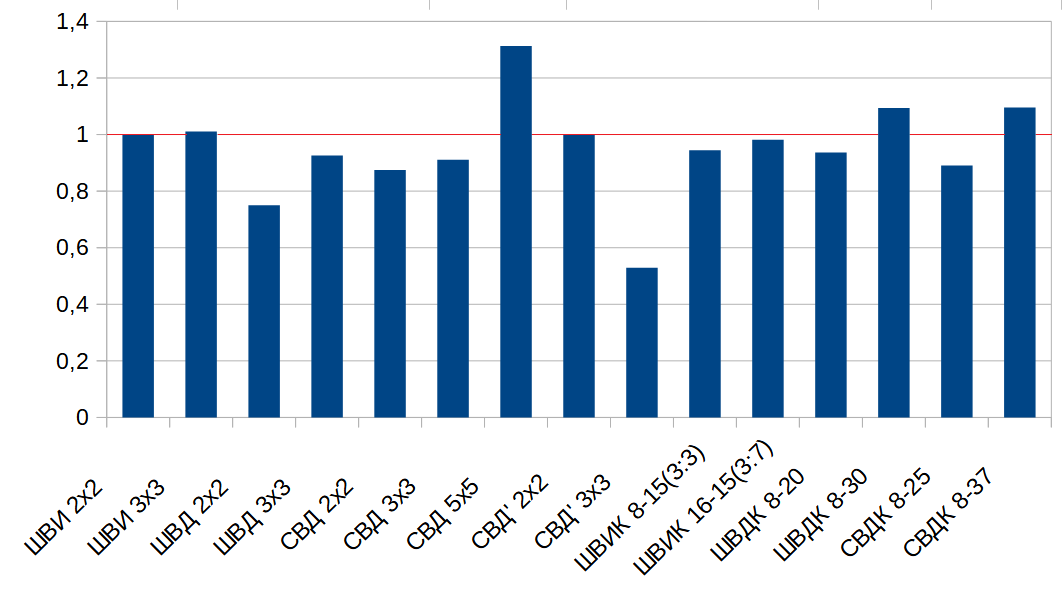
\includegraphics[width=0.6\linewidth]{ratio.png}}
\caption{Отношение длительности вычислений с фиксацией первой координаты к исходной длительности вычислений}
\label{ris:ring}
\end{figure}

Из проведенных экспериментов можно сделать следующие выводы:
\begin{itemize}
  \item Разработанная в рамках данной работы реализация ДЭ показывает конкурентоспособные результаты по сравнению с коммерческим решателем BARON.
  \item Учет симметрии задачи~(\ref{eq:task1}), как правило, позволяет ускорить работу решателя BARON.
\end{itemize}

\section{Заключение}\label{sec:conclusion}

В рамках данной работы была разработана гибридная реализация алгоритма дифференциальной эволюции и градиентного алгоритма. Показано, что разработанная реализация ДЭ демонстрирует конкурентоспособные результаты.

В целях ускорения работы алгоритмов для рассмотренных задач была применена методика анализа наличия группы непрерывных симметрий, в результате которой было обнаружено наличие только фазовой симметрии. Было произведено сравнение гибридного алгоритма и коммерческий решателей с учетом обнаруженной симметрии и без. Выявлено, что учет симметрии может привести к ускорению работы некоторых решателей.


\section*{Приложение}\label{sec:sym}
\subsection*{Линейные симметрии задачи квадратичного программирования}\label{sec:sym:mod}

Решение и анализ задач математического программирования могут быть упрощены при наличии симметрий этих задач, соответствующих некоторым линейным преобразованиям. В частности, знание таких симметрий может быть использовано для уменьшения размерности задачи, ограничения пространства поиска или получения нового локального оптимума из имеющегося.
В настоящей работе исследуется случай непрерывной области решений. В то время как предыдущие исследования симметрии в математическом программировании обычно имели дело с перестановками координат пространства решений~\cite{Kolokolov2012,KWM19,L12}, здесь рассматривается б\'{о}льшая группа обратимых линейных преобразований. Мы изучаем частный случай задачи квадратичного программирования с квадратичными ограничениями в~${\mathbb R}^N$: целевая функция и ограничения задаются квадратичными формами $\textbf{G}, $ и $\textbf{H}_1,\dots,\textbf{H}_n,$ в виде~(\ref{eq:task2}). Следует отметить, что все матрицы $\textbf{G}, $ и $\textbf{H}_1,\dots,\textbf{H}_n,$ симметричны и $\textbf{H} = \sum_{i=1}^{N}\textbf{H}_i$ положительно определена.
Без потери общности будем считать, что все ограничения заданы неравенствами~$\le$.

Под симметрией задачи~(\ref{eq:task2}) подразумевается линейное преобразований
%of the column space
\begin{equation}
\label{eq:Lin}
\textbf{x} \to \textbf{y}=\textbf{Px} \, ,
\end{equation}
%

определенное невырожденной матрицей $\textbf{P}$, такой что задача~(\ref{eq:task2}), выраженная в терминах преобразованного пространства
(т.е, через вектор-столбец $\textbf{y} $), совпадает с исходной задачей. Таким образом, в терминах вектора $\textbf{y}$ задача~(\ref{eq:task2}) формулируется в той же форме.
%
\begin{equation}
\label{eq:Tinit}
\left\{
\begin{array}{l}
\displaystyle
\textbf{y}^T \textbf{G y} \to {\max} \, , \\
\displaystyle
\textbf{y}^T\textbf{H}_1\textbf{y} \le  1 \, , \\
\displaystyle
\dots \\
\textbf{y}^T\textbf{H}_N\textbf{y} \le 1 \, ,
\end{array}
\right.
\end{equation}
%
\textit{с той же самой} матрицей $\textbf{G} $ и тем же набором матриц $\{\textbf{H}_k, k = \overline{1,N}\}$.

В~\cite{yurkov:symmetry} показано, что симметричная матрица~$\textbf{H} = \sum_{k=1}^{n}\textbf{H}_k, k = \overline{1,N}$ может быть представлена как конгруэнтное преобразование диагональной матрицы:
%
\begin{equation}
\label{eq:BSSTDS}
\textbf{H}=\textbf{S}^T\textbf{DS} \, ,
\end{equation}
%
где $\textbf{D}$ -- диагональная матрица, которая может иметь только ``0'', ``1'', или ``-1'' на ее главной диагонали. Матрица $\textbf{S}$ Может быть получена конструктивно, например, конечным методом Лагранжа~(\cite{Lancaster},~Г.~5).

Матрица $\textbf{S}$ описывает переход в группу ортогональных преобразований, в которой производится поиск подгрупп непрерывных симметрий.
Любой ее элемент такой группы может быть выражен с помощью базисных элементов, называемых генераторами:
%
\begin{equation}
\textbf{X} = \sum_k a_k G_k \, ,
\end{equation}
%
где $ a_k $ являются вещественными числами, $G_k $ являются генераторами. Пространство кососимметричных матриц имеет размерность $N(N-1)/2$, а количество коэффициентов $a_k$ будет равно количеству генераторов. В качестве генераторов можно выбрать матрицы, у которых над главной диагональю все элементы равны~0, кроме одного элемента, равного~1. Тогда кососимметрия однозначно определяет остальные матричные элементы этих генераторов. Итак, любой элемент $Q$ из $SO(N)$ можно представить в виде:
%
\begin{equation}
\label{eq:sunexp}
\textbf{Q}=e^{\sum_k a_k G_k} \, .
\end{equation}
%

Сам поиск осуществляется решением системы линейных уравнений~(\ref{eq:commutat2}):

%
\begin{equation}
\label{eq:commutat2}
\left\{
\begin{array}{l}
\displaystyle
\tilde{\textbf{H}}_n \left(\sum\limits_ka_kG_k\right) =
\left(\sum\limits_ka_kG_k\right) \tilde{\textbf{H}}_n \, , \\ \\
\displaystyle
\tilde{\textbf{G}} \left(\sum\limits_ka_kGk\right) = \left(\sum\limits_ka_kG_k\right) \tilde{\textbf{G}} \, .
\end{array}
\right.
\end{equation}
%

Уравнения~(\ref{eq:commutat2}) представляют собой систему линейных алгебраических уравнений, определяющих параметры $a_k$. Эта система однородна, поэтому она имеет континуум ненулевых решений или одно тривиальное решение. Тривиальное нулевое решение всегда присутствует и соответствует единичной матрице $\textbf{Q}$. Некоторые из параметров $a_k$ остаются ``свободными'' (это будут параметры искомой подгруппы), а остальные из~$a_k$ могут быть линейно выражены через ``свободные''. Решение этой системы уравнений~(\ref{eq:commutat2}) может быть получено конструктивно методом Гаусса.

Условие инвариантности задачи относительно преобразования~$\textbf{Q}$ превращается в
%
\begin{equation}
\label{eq:subG1}
\textbf{Q}=e^{\sum_k a_k \hat{G}_k} \, ,
\end{equation}
%
где сумма идет по <<свободным>> параметрам $a_k$, а новые генераторы, обозначаемые через~$\hat{G}_k$, являются линейными комбинациями прежних генераторов~$G_k$. Множество всех $\textbf{Q}$-матриц, удовлетворяющих~(\ref{eq:subG1}), параметризуется конечным набором вещественных параметров $a_k$.

\subsection*{Поиск группы непрерывных симметрий  задаче оптимизации направленности фазированных антенных решеток}\label{sec:sym:exp}

Вычислительный эксперимент состоит из следующих этапов:
\begin{enumerate}
  \item Обработка. На этом этапе возможная неточность данных нивелируется усреднением симметричных компонент матриц (матрицы $\textbf{G}$ и $\textbf{H}$ должны быть симметричны).
  \item %Normalization of matrices $B_i$.
  Преобразование $ {\textbf{H}}_{\Sigma} = \sum_{i} \textbf{H}_i$ к канонической форме используя метод Лагранжа для вычисления матриц~$\textbf{S}$ и $\textbf{S}^{-1} $.
  \item Применение метода Гаусса к системе линейных уравнений~(\ref{eq:commutat2}) для вычисления генераторов~$\hat{G}_n$.
\end{enumerate}

Следует отметить, что входные данные могут содержать некоторые погрешности, которые приводят к несимметричности матриц $\textbf{G}$ и $\textbf{H}$, что может существенно повлиять на поиск непрерывных групп симметрий. Таким образом, на этапе~1, мы используем известные свойства задачи чтобы нивелировать влияние погрешности.
Также, в методе Гаусса на шаге 3, любые значения принимаются за 0 если их абсолютное значение меньше определенного порогового значения~$\Delta$, который является параметром алгоритма. Причина в том, что последовательное исключение переменных из уравнений, выполняемое методом Лагранжа с представлением вещественных чисел с плавающей запятой, не может гарантировать идеальную точность.
В результате некоторые линейно зависимые строки матрицы не могут быть исключены, что может привести к неверному результату.
%To eliminate this effect, a threshold error is introduced.
Большое значение порога~$\Delta$ может привести к вырожденности задачи, тогда как слишком малое значение~$\Delta$ не позволит выявить линейные зависимости.

В данном эксперименте, $\Delta$ изменялось от $ 10^{-4} $ до $ 10^{-12} $. В данном диапазоне для каждого рассмотренного частного случая задачи, не было получено различий в полученных решениях.

%\subsection{Optimization of the Excitation of Antenna Arrays}

Описанная процедура нахождения непрерывных групп симметрий применяется к примерам, описанным в~\cite{tyunin:daor}. Для всех рассмотренных задач было выявлено только наличие симметрии относительно преобразования $\textbf{i} \to e^{\emph{\textbf{j}}\phi}\textbf{i}$ всех комплексных координат (по произвольному углу~$\phi$). За $\emph{\textbf{j}}$ здесь обозначена мнимая единица. Данная симметрия находит применение для уменьшения размерности области поиска на единицу. Например, фиксируя $Im(y_{N})=0$, что эквивалентно добавлению ограничения $x_{2N}=0$ к задаче~(\ref{eq:task2}). Возможно, множественность решений объясняется наличием дискретных симметрий. Выявление дискретных симметрий является объектом дальнейших исследований.

В результате работы алгоритма было выявлено, что все генераторы~$\hat{G_k}$ могут быть выражены через один новый генератор вида
$$
\hat{G} = \left(\begin{array}{cccccccc}
        0 & 0 & 0 & 0 & -1 & 0 & 0 & 0\\
        0 & 0 & 0 & 0 & 0 & -1 & 0 & 0\\
        0 & 0 & 0 & 0 & 0 & 0 & -1 & 0\\
        0 & 0 & 0 & 0 & 0 & 0 & 0 & -1\\
        1 & 0 & 0 & 0 & 0 & 0 & 0 & 0\\
        0 & 1 & 0 & 0 & 0 & 0 & 0 & 0\\
        0 & 0 & 1 & 0 & 0 & 0 & 0 & 0\\
        0 & 0 & 0 & 1 & 0 & 0 & 0 & 0
\end{array}\right),
$$
который соответствует фазовой симметрии. Для данного генератора при $a = 1$
$$e^{a\hat{G}} = \left(\begin{array}{cccccccc}
        0.5403 & 0 & 0 & 0 & -0.8415 & 0 & 0 & 0\\
        0 & 0.5403 & 0 & 0 & 0 & -0.8415 & 0 & 0\\
        0 & 0 & 0.5403 & 0 & 0 & 0 & -0.8415 & 0\\
        0 & 0 & 0 & 0.5403 & 0 & 0 & 0 & -0.8415\\
        0.8415 & 0 & 0 & 0 & 0.5403 & 0 & 0 & 0\\
        0 & 0.8415 & 0 & 0 & 0 & 0.5403 & 0 & 0\\
        0 & 0 & 0.8415 & 0 & 0 & 0 & 0.5403 & 0\\
        0 & 0 & 0 & 0.8415 & 0 & 0 & 0 & 0.5403
\end{array}\right).
$$

\bibliography{external}
\end{document}
